% LaTeX file for a 1 page document
\documentclass[12pt]{article}
\usepackage{amsmath}
\usepackage{amssymb}
\usepackage{amsthm}
%\usepackage{physymb}
\usepackage{graphicx}
%\usepackage{wrapfig}
\usepackage{tikz}
\usetikzlibrary{calc,patterns,decorations.pathmorphing,decorations.markings}

\title{EP 222 Assigment 2}
\date{October 10, 2013}
\author{Manish Goregaokar (120260006)}

\begin{document}
\maketitle

\section{Question 1}

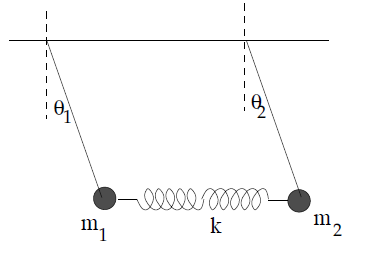
\includegraphics[scale=1]{1.png}


We shall take $\theta_1,\theta_2$ as our coordinates. Let the rigid supports be of length $l$, and let the distance between the supports be equal to the equilibrium length of the spring, $d$. The kinetic energy of this system is $T=\frac{l^2}2(m_1\dot\theta_1^2+m_2\dot\theta_2^2)$\\
Rewriting $T$ as a matrix, $\mathbf T=[t_{ij}]=\left[\frac{\partial^2 T}{\partial \dot\theta_i\partial \dot\theta_j}\right]=l^2\begin{pmatrix}
m_1 & 0\\
0 & m_2
\end{pmatrix}$\\

The potential energy is \begin{align}V &=& &m_1gl(1-\cos\theta_1)+m_2gl(1-\cos\theta_2)+\frac12k(l(\theta_2-\theta_1))^2\notag\\ &\approx & &m_1gl\theta_1^2 +m_2gl\theta_2^2+\frac12kl^2(\theta_1^2+\theta_2^2+2\theta_1\theta_2)\notag
\end{align}
\\ Rewriting $V$ as a matrix, \begin{align}\mathbf V &=& &[V_{ij}]\notag\\ &=& &\left[\frac{\partial^2 V}{\partial \theta_i\partial \theta_j}\right]\notag\\ &=& &\begin{pmatrix}
2m_1gl+kl^2 & -kl^2\\
-kl^2 & 2m_2gl+kl^2
\end{pmatrix}\notag
\end{align}\\
Now, the normal mode frequencies are given by the eigenvalue equation $$|\mathbf V-\omega^2\mathbf T|=0$$

$$\therefore\left|\begin{pmatrix}
2m_1gl+kl^2 & -kl^2\\
-kl^2&  2m_2gl+kl^2
\end{pmatrix}-\omega^2l^2\begin{pmatrix}
m_1 &0\\0&m_2
\end{pmatrix}\right|=0$$
Rewriting $\lambda=\omega^2l^2$
\begin{align}
&\therefore \begin{vmatrix}k l^2+2 g m_1 l-\lambda  m_1 & k l^2 \\
 k l^2 & k l^2+2 g m_2 l-\lambda  m_2 \\
\end{vmatrix} &=& 0\notag\\ &\implies 4 g^2 l^2 m_1 m_2+2 g k l^3 m_1+2 g k l^3 m_2\notag\\ &-4 g \lambda  l m_1 m_2-k \lambda  l^2 m_1-k \lambda  l^2 m_2+\lambda ^2 m_1 m_2 &=& 0\notag 
\end{align}	

From this we get roots for $\lambda$ as $2gl$ and $\frac{kl^2}{\mu}+2gl$, so the normal modes are $\boxed{\omega=\sqrt{2\frac{g}{l}}}$ anand $\boxed{\omega=\sqrt{2\frac{g}{l}+\frac{k}{\mu}}}$ where $\mu$ is the reduced mass.\\

The eigenvectors can be found by solving $\mathbf{VA}=\omega^2\mathbf{TA}$. This expands to $$\begin{pmatrix}
 2 g l m_1+k l^2 & -k l^2 \\
 -k l^2 & 2 g l m_2+k l^2 \\
\end{pmatrix}
\begin{pmatrix}
 A_1 \\
 A_2 \\
\end{pmatrix}
=\lambda 
\begin{pmatrix}
 m_1 & 0 \\
 0 & m_2 \\
\end{pmatrix}
\begin{pmatrix}
 A_1 \\
 A_2 \\
\end{pmatrix}
$$

which gives rise to eigenvectors $\boxed{\mathbf A= \begin{pmatrix}1 \\ 1\end{pmatrix},\begin{pmatrix}m_2 \\ -m_1\end{pmatrix}}$, or relative amplitudes ($\theta_2:\theta_1$) $1$ and $-\frac{m_1}{m_2}$.

\section{Question 2}
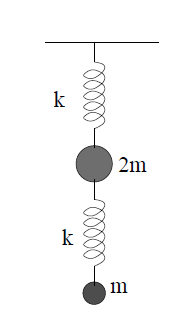
\includegraphics[scale=1]{2.png}

Our generalized coordinates shall be the elongations in each spring, $x_1,x_2$ ($x_1$ is for the upper spring).\\
The velocities of the masses are $\dot x_1$ for $2m$ and $\dot x_1 +\dot x_2$ for $m$.\\
$\therefore T=\frac12 2m \dot x_1^2 + \frac12 m (\dot x_1+\dot x_2)^2=\frac12(3m\dot x_1^2 + m\dot x_2^2+2m\dot x_1\dot x_2)$\\
Rewriting $T$ as a matrix, $\mathbf T=[t_{ij}]=\left[\frac{\partial^2 T}{\partial \dot x_i\partial \dot x_j}\right]=\frac{m}2\begin{pmatrix}
6 & 2\\
2 &2
\end{pmatrix}$\\
The potential energy is simply $\frac12(kx_1^2+kx_2^2)-2mg(l_1+x_1)-mg(l_1+x_1+l_2+x_2)$ ($l_1,l_2$ are natural lengths of springs), giving $\mathbf V=[V_{ij}]=\left[\frac{\partial^2 V}{\partial x_i\partial x_j}\right]=\frac{k}2\begin{pmatrix}
2 & 0\\
0 &2
\end{pmatrix}$\\
Now, the normal mode frequencies are given by the eigenvalue equation $$|\mathbf V-\omega^2\mathbf T|=0$$
$$\therefore\left| \frac{k}2\begin{pmatrix}
2 & 0\\
0 &2
\end{pmatrix}-\omega^2\frac{m}2\begin{pmatrix}
6 & 2\\
2 &2
\end{pmatrix}\right|=0$$
Rewriting $\lambda=\omega^2\frac{m}{k}$
\begin{align}
&\therefore \begin{vmatrix}
2 -6\lambda & 0-2\lambda\\
0-2\lambda &2-2\lambda
\end{vmatrix} &=& 0\notag \\
&\implies (2-6\lambda)(2-2\lambda)-(-2\lambda)^2 &=& 0\notag\\
&\implies  8\lambda^2 -16\lambda +4 &=& 0\notag\\
&\implies  2\lambda^2 -4\lambda +1 &=& 0\notag\\
&\implies \lambda &=& \frac{4\pm\sqrt{16-8}}{4}\notag\\
&~ &=& 1\pm\frac1{\sqrt{2}}\notag\\
&\implies \omega &=&\sqrt{\frac{k}{m}\left(1\pm\frac1{\sqrt{2}}\right)}\notag
\end{align}

Thus, the normal modes are $\boxed{\omega_1=\sqrt{\frac{k}{m}\left(1+\frac1{\sqrt{2}}\right)},~~\omega_2=\sqrt{\frac{k}{m}\left(1-\frac1{\sqrt{2}}\right)}}$
\section{Question 3}
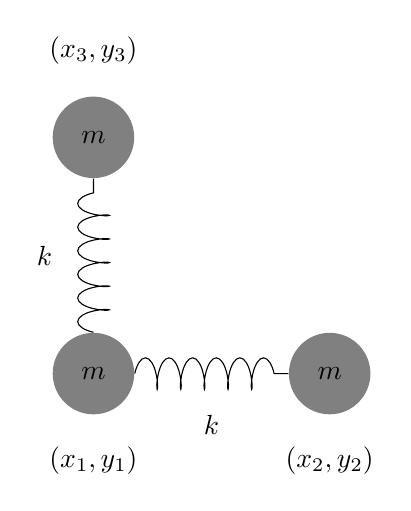
\begin{tikzpicture}
\node[circle,fill=gray,inner sep=2.5mm] (a) at (0,3) {$m$};
\node[above=0.1cm, above of= a] {$(x_3,y_3)$}; 
\node[circle,fill=gray,inner sep=2.5mm] (b) at (0,0) {$m$};\node[below=0.1cm, below of= b] {$(x_1,y_1)$} ;
\node[circle,fill=gray,inner sep=2.5mm] (c) at (3,0) {$m$}; \node[below=0.1cm, below of= c] {$(x_2,y_2)$};
\draw[decoration={aspect=0.3, segment length=3mm, amplitude=2mm,coil},decorate] (b) -- (a) node [midway, left=0.4cm] {$k$}; 

\draw[decoration={aspect=0.3, segment length=3mm, amplitude=2mm,coil},decorate] (b) -- (c)  node [midway, below=0.4cm] {$k$}; 
\end{tikzpicture}\\
 Let $q_1,q_2,q_3$ be the $x$ coordinates, and $q_4,q_5,q_6$ be the y coordinates.

The kinetic energy is $T=\frac{m}2(\sum \dot q_i^2)$, giving $\mathbf T=[t_{ij}]=\left[\frac{\partial^2 T}{\partial \dot q_i \dot q_j}\right]=m\mathbf I$, where $\mathbf I$ is the 6$\times$6 identity matrix.

\newcommand{\dxsq}[2]{(x_#1-x_#2)^2}
\newcommand{\dysq}[2]{(y_#1-y_#2)^2}
The potential energy is $$V=\frac{k}2\left(\left(\sqrt{\left(x_1-x_2\right){}^2+\left(y_1-y_2\right){}^2}-a\right){}^2+\left(\sqrt{\left(x_3-x_1\right){}^2+\left(y_3-y_1\right){}^2}-a\right){}^2\right)$$. This gives us a matrix $\mathbf V=[V_{ij}]=\left[\frac{\partial^2 V}{\partial q_i  q_j}\right]$, which when expanded gives us an unprintably large matrix. However, on substituting the equilibrium values of the coordinates, we get the much more manageable
$$\frac{k}2\begin{pmatrix}

 2 & -2 & 0 & 0 & 0 & 0 \\
 -2 & 2 & 0 & 0 & 0 & 0 \\
 0 & 0 & 0 & 0 & 0 & 0 \\
 0 & 0 & 0 & 2 & 0 & -2 \\
 0 & 0 & 0 & 0 & 0 & 0 \\
 0 & 0 & 0 & -2 & 0 & 2 \\


\end{pmatrix}$$

Now, the eigenvalue equation is $|\mathbf V-\omega^2 \mathbf T|=0$, giving us $$\left|\frac{k}{2}\begin{pmatrix}
 2 & -2 & 0 & 0 & 0 & 0 \\
 -2 & 2 & 0 & 0 & 0 & 0 \\
 0 & 0 & 0 & 0 & 0 & 0 \\
 0 & 0 & 0 & 2 & 0 & -2 \\
 0 & 0 & 0 & 0 & 0 & 0 \\
 0 & 0 & 0 & -2 & 0 & 2 \\
\end{pmatrix}-\omega^2 m\mathbf I\right|=0$$
Writing $\lambda=\frac{2m\omega^2}{k}$
$$\therefore\begin{vmatrix}

 2-\lambda  & -2 & 0 & 0 & 0 & 0 \\
 -2 & 2-\lambda  & 0 & 0 & 0 & 0 \\
 0 & 0 & -\lambda  & 0 & 0 & 0 \\
 0 & 0 & 0 & 2-\lambda  & 0 & -2 \\
 0 & 0 & 0 & 0 & -\lambda  & 0 \\
 0 & 0 & 0 & -2 & 0 & 2-\lambda  \\


\end{vmatrix}=0$$
$$\therefore \lambda ^2 \left(\lambda ^4-8 \lambda ^3+16 \lambda ^2\right)=0$$
   $$\therefore (\lambda -4)^2 \lambda ^4=0$$
   
   
   This gives us eigenvalues $\lambda=0,0,0,0,4,4$. Thus, the normal modes are $\boxed{\sqrt{2\frac{k}{m}} }$ with multiplicity 2.
\section{Question 4}
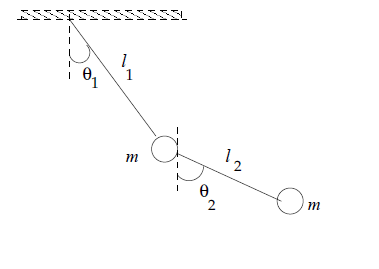
\includegraphics[scale=1]{4.png}

We shall take our coordinates as $\theta_1,\theta_2$. The velocity of the upper bob is $\frac12ml_1^2\dot\theta_1^2$. For the second bob, its position is $\mathbf r_2=l_1(\cos\theta_1\hat i +\sin\theta_1\hat j)+ l_2(\cos\theta_2\hat i +\sin\theta_2\hat j)$.  This gives us velocity $$\dot{\mathbf{r_2}}=l_1\dot\theta_1(-\sin\theta_1\hat i +\cos\theta_1\hat j)+ l_2\dot\theta_2(-\sin\theta_2\hat i +\cos\theta_2\hat j)$$, which can be rewritten as $$\dot{\mathbf{r_2}}=\hat i(-l_1\dot\theta_1\sin\theta_1-l_2\dot\theta_2\sin\theta_2)+ \hat j(l_1\dot\theta_1\cos\theta_1+l_2\dot\theta_2\cos\theta_2)$$. The kinetic energy $$T=\frac12ml_1^2\dot\theta_1^2+\frac12m|\dot{\mathbf{r_2}}|^2=\frac12m\left(2\dot{\theta }_1^2 l_1^2+\dot{\theta }_2^2
   l_2^2+2 \dot{\theta }_2 \dot{\theta }_1 l_1
   l_2 \cos \left(\theta _1-\theta _2\right)\right)$$
   
Rewriting as a matrix,  $$\mathbf T=[t_{ij}]=\left[\frac{\partial^2 T}{\partial \dot \theta_i \dot \theta_j}\right]=m\begin{pmatrix}
2l_1^2 & l_1l_2\cos(\theta_1-\theta_2)\\
l_1l_2\cos(\theta_1-\theta_2) & l_2^2
\end{pmatrix}$$
Near equilibrium ($\theta_1,\theta_2=0$), $\mathbf T=\begin{pmatrix}
2l_1^2 & l_1l_2\\
l_1l_2 & l_2^2
\end{pmatrix}$\\

The potential energy $V=-mgl_1\cos\theta_1-(mgl_1\cos\theta_1+mgl_2\cos\theta_2)$. This gives us a potential matrix $$\mathbf V =\left[\frac{\partial^2 V}{\partial \theta_i \theta_j}\right]=\begin{pmatrix}
2mgl_1\cos\theta_1&0\\
0& mgl_2\cos\theta_2
\end{pmatrix}$$

which, at equilibrium, is $mg\begin{pmatrix}
2l_1&0\\0&l_2
\end{pmatrix}$

The eigenvalue equation is $|\mathbf V-\omega^2 \mathbf T|=0$, which comes out to be $$\left|mg\begin{pmatrix}
2l_1&0\\0&l_2
\end{pmatrix}-\omega^2\begin{pmatrix}
2l_1^2 & l_1l_2\\
l_1l_2 & l_2^2
\end{pmatrix}\right|=0$$

With $\lambda=\frac{\omega^2}{mg}$, we get

\begin{align*}
&\left|\begin{pmatrix}
2l_1&0\\0&l_2
\end{pmatrix}-\lambda\begin{pmatrix}
2l_1^2 & l_1l_2\\
l_1l_2 & l_2^2
\end{pmatrix}\right| &=0\notag\\
&\therefore \lambda ^2 l_2^2 l_1^2-2 \lambda  l_2 l_1^2-2 \lambda  l_2^2 l_1+2 l_2 l_1 &=0 \notag\\
&\therefore \lambda &= \frac{l_1+l_2\pm\sqrt{l_1^2+l_2^2}}{l_1 l_2}\notag\\
&\therefore \omega &= \sqrt{mg\frac{l_1+l_2\pm\sqrt{l_1^2+l_2^2}}{l_1 l_2}}\notag
\end{align*}

To find the eigenvectors, we solve $\mathbf {VA}=\omega^2\mathbf{TA}$, which expands to $$\begin{pmatrix}
2l_1&0\\0&l_2
\end{pmatrix}\begin{pmatrix}
A_1\\A_2
\end{pmatrix}=\lambda\begin{pmatrix}
2l_1^2 & l_1l_2\\
l_1l_2 & l_2^2
\end{pmatrix}\begin{pmatrix}
A_1\\A_2
\end{pmatrix}$$

This gives us eigenvectors $$\mathbf A= \begin{pmatrix}
l_2 \left(\pm(l_1+l_2)+\sqrt{l_1^2+l_2^2}\right)\\
-2 l_1 \left(\sqrt{l_1^2+l_2^2}\pm l_1\right)
\end{pmatrix}$$

These are already orthogonal ($\mathbf A_1^T\mathbf{TA_2}=0$). On normalizing them ($\mathbf A_i^T\mathbf{TA_i}=1$), we get $$\boxed{\mathbf A=\frac1{2 l_1 l_2 \sqrt{l_1^2\pm  l_1\sqrt{l_1^2+l_2^2}+l_2^2}}\begin{pmatrix}
l_2 \left(\pm(l_1+l_2)+\sqrt{l_1^2+l_2^2}\right)\\
-2 l_1 \left(\sqrt{l_1^2+l_2^2}\pm l_1\right)
\end{pmatrix}}$$ for corresponding normal modes $\boxed{ \omega = \sqrt{mg\frac{l_1+l_2\pm\sqrt{l_1^2+l_2^2}}{l_1 l_2}}}$
\end{document}
}
